% !TEX encoding = UTF-8 Unicode
% -*- program: pdflatex -*-
\documentclass[fleqn,10pt,lineno]{wlpeerj}
\usepackage[hidelinks]{hyperref}
\usepackage[T1]{fontenc}
\usepackage{tgtermes}
\usepackage{etoolbox}
\usepackage{graphicx}
\usepackage{subfloat}
\usepackage{comment}
 \usepackage{lscape}
\usepackage{soul}
\hypersetup{
   pdftitle={CVX},
   pdfauthor={Alexa Tyszka, Karolis Ramanauskas, Boris Igi{\'c}}
   }
%\usepackage[all]{hypcap} % NOTE BELOW:
%B: I don't know where this comes from (or who put it here, me, K, A?), but K says it breaks \includegraphics
% If it is used for something important, let me know.
\usepackage{doi} % remove url!
\graphicspath{{figures/}}
\renewcommand{\bibsection}{\section*{References}}
\providecommand{\e}[1]{\ensuremath{\times 10^{#1}}}
\newcommand{\ca}{\textit{ca}.}

%--------------------------------------------------
% How to Handle Supplemental Materials
%--------------------------------------------------

% PeerJ instructions:
%
% Supplemental materials. Online publishing allows inclusion of information that may not fit into a printed paper with page limits or may be deemed redundant (tables of data included in a figure) or otherwise inappropriate for the print version (extensive photographic evidence, metadata, other potentially useful information not essential to the paper). These files are not included in the page/word counts of the manuscript and will be presented online as submitted by the authors (not copy edited). Authors should upload this information as a separate file entitled ?Supplement? in PeerTrack. Text references to this material in the manuscript will be inserted as hotlinks to the online information. Supplemental figure and table numbers should be preceded by the letter S to indicate supplemental (Supplemental Table S1, Supplemental Fig. S4).
%
% Here's what we'll do:
% (1) we'll have another tex file called cvx-cactaceae-suppinfo.tex and we'll insert it for use in this file as follows:
% \externaldocument{cvx-cactaceae-suppinfo.tex}
%
% (2) each figure table will be inserted as usual with \begin{figure} ... \end{figure}
% (3) In the text, you just reference these with their label, as you would any other figure! That's it!

%--------------------------------------------------
% TITLE PAGE
%--------------------------------------------------
\title{Genome evolution, taxonomy, and transmission of potexviruses in cacti (\textit{Alphaflexiviridae})}

\author[1,$\dagger$]{Alexa Tyszka}
\author[1]{Karolis Ramanauskas}
\author[1]{Boris Igi\'c}
\affil[1]{Department of Biological Sciences, University of Illinois at Chicago, 840 West Taylor St.\ MC067, Chicago, IL 60607, United States of America}
 \affil[$\dagger$]{Author for correspondence.}


%\begin{linenumbers}
%\modulolinenumbers[1]
%\setstretch{1.0}

%--------------------------------------------------
% ABSTRACT 
%--------------------------------------------------

\begin{abstract}

\textit{Potexvirus} is a group of positive-sense single-stranded RNA viruses known to infect many flowering plants, including cacti (Cactaceae).
The current viral taxonomic naming schemes in this group often employ informal or outdated host plant names (synonyms), which complicate systematic study.
One such group, often named with a suffix "Virus X," presents a further complication---nearly all of its published sequences are from infections of cultivated plants, in which infections may dramatically affect yield.
Because their host-specificity is broad, the source of infections, the natural distribution of this group, and the significance of infections in wild species of cacti all remain unclear.
The lack of clarity is partly related to low sampling across the Potexviruses that infect cacti. 
And yet, the availability of sampled plant transcriptomes, all of which are practically metatranscriptomes, has recently exploded, along with the decreasing expense and difficulty of conducting RNAseq experiments.
Here, we harness these new tools and perform phylogenetic analyses aimed at clarifying taxonomic diversity, quantifying patterns of tissue expression, diversity, and examining selective pressures across viral genomes. 
The results suggest a novel mode of transmission by sex (pollination) for this viral group, based on significant expression in pollen.
We examine and discuss the implications of our key results for the taxonomy of \textit{Potexviruses} that infect Cactaceae, noting their vastly understudied ecological significance.

\end{abstract}

%--------------------------------------------------
\begin{document}
%--------------------------------------------------
%
\flushbottom
\maketitle
\thispagestyle{empty}
%\setlength{\emergencystretch}{7.5pt}
%\setstretch{1.0}
%\setlength{\parindent}{0.25in}


%--------------------------------------------------
\section*{Introduction}
%--------------------------------------------------

Molisch's (1885) \nocite{molisch1885} discovery of ``protein bodies'' on several species of cacti was one of the first documented descriptions of viruses.
For nearly a century, subsequent comparative study of viruses remained limited to direct observational data of gross morphology, augmented with clever experimental approaches, such as filtration and inoculation \citep{mettenleiter2017}.
A transformative advancement in virology---and all of biology---has been the advent of massively parallel DNA and RNA sequencing. 
The rapidly improving sequencing tools enable rapid identification of organisms from seemingly any sampled surface of the Earth.
One common thread is that virtually every macro-organism genome study uncovers a micro-organismal metagenome, composed of both targeted host sequences and those from myriad co-existing organisms. 
Metagenomic studies have yielded an enormous number of genomes and have vastly expanded the global viriome \citep{gregory_marine_2019,lefeuvre2019,shi_redefining_2016}. 
%B: this is an unusually large in-line citation set. I would pick one or two transformative studies, not the whole gamut.
The unprecedented amount of data resulting from metagenomic studies has also caused significant policy changes and revisions by the International Committee on Taxonomy of Viruses (ICTV) policy \citep{ictv2020,simmonds2017virus}, but nearly all viruses remain named by their original description of host, location, and/or symptoms.

Historic naming conventions are ill-suited for host plants whose own taxonomic placement is uncertain, which has been particularly true for rapidly diversified groups such as Cactaceae (cacti).
Molisch's ``protein bodies'' are now widely understood to be comprised of plant-infecting potexviruses (\textit{Tymovirales}, family \textit{Alphaflexiviridae}).
Their positive-sense, single-stranded RNA genomes consist of 5.9-7.0 kb of positive-sense single-stranded RNA \citep{martelli_family_2007}.
Generally presenting as elongated, rod-shaped filamentous viruses, they express five primary open reading frames (ORFs): Replicase (Rep), Triple gene block (TGB), Coat protein (CP), coded in the 5' direction as well as two smaller overlapping ORFs coded in the 3' direction: ORF6 and ORF7 \citep{martelli_family_2007}. 
%if one of these citations mentions the structure, it is sufficient.
%at: deleted all but the most relevant citation
%They are closely related to other \textit{Potexviruses} such as \textit{Alternantha Mosaic Virus} and \textit{Papaya Mosaic Virus} \citep{martelli_family_2007,park_detection_2018,liou_complete_2004}.
Members of this group produce variably symptomatic infections in cacti, and many infected plants show no external signs of viral infection \citep{bos_symptoms_1977, liou_complete_2004}. 
Neither the significance of their infections in nature, nor relative modes of transmission are clear. 
Reports of symptomatic plants range from 0\%-5.5\% in wild species in the southwestern United States \citep{attathom_occurrence_1978} to 44\% in agricultural fields on Hainan Island, China \citep{peng_molecular_2016}.
The most commonly recognized symptoms of the disease are mosaic, mottling, stunted growth, and distortion \citep{attathom_occurrence_1978, maliarenko_cactus_2013, peng_molecular_2016}.
Infection through grafting and mechanical contact, particularly following stem injury and human-mediated or hemipteran insect-mediated sap inoculation, is well-documented \citep{liou_complete_2004,maliarenko_cactus_2013,park_detection_2018}.
Grafting is a primary means of propagation among crop cacti \citep{park_detection_2018}, and \textit{Selenicereus} is a commonly chosen graft stock.
However, there are reports of other members within the family \textit{Alphaflexiviridae} transmitting via insect and seed vectors \citep{martelli_family_2007}, and pre-DNA studies tentatively suggest that in the wild, pollen may transmit CVX \citep{attathom_occurrence_1978}.

Viral taxonomy is complicated by many aspects of biology and taxonomic practices.
\textit{Schlumbergera truncata} (Haworth) Moran has undergone a number of name changes, including \textit{Epiphyllum truncatum} Haworth in 1819, \textit{Cactus truncatus} (Haworth) Link in 1822, and \textit{Zygocactus truncatus} (Haworth) K. Schumann in 1890, dramatically confusing subsequent viral taxonomy.
%This naming scheme may cause confusion as it results in many distinct viruses having the same name.
Thus, currently accepted names in the \textit{Potexvirus} group include \textit{Cactus Virus X} (CVX), \textit{Zygocactus Virus X} (ZyVX), and \textit{Schlumbergera Virus X} (SchVX), each of which was likely characterized on the same host genus (and possibly species). %cite
The Baltimore classification system standardizes viral classification by intrinsic morphological characteristics of a virus' replication machinery. 
It has been integrated into the ICTV guidelines to better reflect viral evolutionary relationships \citep{ictv2020}.
The term ``plant virus'' in itself is problematic since there is strong evidence to suggest that many viruses have transitioned from fungal or invertebrate hosts to plant hosts \citep{lefeuvre2019}. %this is possibly important and I have not read the paper. The interpretation of possibility of spillover is critical. Make sure that there are documented cases where a species jumps host across this chasm!
Additionally, many plant viruses that infect agriculturally important species are named using the common name of a plant, which carries its own problems, for example: \textit{Pitaya Virus X} is named for the common name ``Pitaya'' which can refer to as many as thirty-one species within the genus \textit{Selenicereus} \citep{korotkova_phylogenetic_2017,guerrero_phylogenetic_2019,le_bellec_12_2011}. 
The matter is further complicated by basic viral ecology, because one virus may infect many hosts, and one host may be co-infected by many viruses. 
Single-stranded RNA viruses have faster rates of evolution than their host plants. %B: just one virus is considered in this whole section?
There is no guarantee that viral evolution and speciation follow linearly behind plant evolution and speciation---especially due to viral host-switching.
These problems persist throughout the genus \textit{Potexvirus} and are especially prominent in cactus-infecting \textit{Potexvirus} species.
We suggest a phylogeny-based approach to remedy some prominent taxonomic issues within this specific clade.

%at: I will trim this down soon and make it introduction-worthy. 
%The species \textit{Cactus Virus X}, \textit{Zygocactus Virus X}, \textit{Schlumbergera Virus X}, \textit{Pitaya Virus X}, and \textit{Opuntia Virus X} are all \textit{Potexviruses} (family Alphaflexiviridae) that are grouped broadly by their infections of certain cacti: \textit{Selenicereus undatus} and \textit{S. polyrhizus} \citep{li_viral_2015,peng_molecular_2016}; \textit{Opuntia spp.} especially \textit{O. tuna} \citep{koenig_molecular_2004, duarte_Potexvirus_2008} and \textit{O. monacantha} \citep{attathom_occurrence_1978} Sammons 1961 Duarte 2008; \textit{Schlumbergera} (previously \textit{Zygocactus}) \textit{truncata} and \textit{S. bridgesii} \citep{duarte_Potexvirus_2008, koenig_molecular_2004}, \textit{Parodia }(previously \textit{Notocactus}) \textit{leninghausii} \citep{park_detection_2018}, \textit{Echinopsis chamaecereus f. cristata}, \textit{E. pectinatus f. cristata}, \textit{E. jusbertii}, and \textit{E. macrogona} \citep{maliarenko_cactus_2013}; \textit{Mammillaria elongata f. cristata} \citep{maliarenko_cactus_2013}; and multiple other species within many genera in the family Cactaceae \citep{evallo_brief_2021}. Of these viruses, only \textit{Cactus Virus X} (CVX) has been reported on wild \textit{Ferocactus cylindraceus} (previously \textit{Ferrocactus acanthodes}) \citep{attathom_occurrence_1978}. 
%However, this report predates DNA records confirming the viral identity.
%Additionally, the viruses are frequently manipulated with serological experiments and have been found to produce lesions (which indicate infection) on: \textit{Chenopodium murale L.} \citep{maliarenko_cactus_2013} and C. quinoa \citep{attathom_identification_1978,attathom_occurrence_1978, brandes_untersuchungen_1963-1}; Nicotiana alata Link el. Otto \citep{maliarenko_cactus_2013}; Four species of Amaranthaceae \citep{attathom_identification_1978}; Escobaria vivipara \citep{attathom_identification_1978}; and other Cactaceae \citep{attathom_identification_1978}.

Knowledge about cactus-infecting \textit{Potexviruses} contributes to a growing yet biased study of plant viruses. 
Human-assisted dispersal, grafting, and cultivation obscure the evolutionary history of these viruses, which parallels the disproportionate sampling representation of plants raised in greenhouses or for agricultural production. 
However, \textit{Cactus Virus X} and associated viruses seem restricted to cactaceous hosts for unknown reasons---every sample of CVX or CVX-related viruses has come from cacti.
The few studies that have investigated wild \textit{Potexviruses} of cacti predate DNA methods and have yet to identify the origin.
Recent sequencing efforts have revealed multiple inconsistent virus-host pairs on cacti.
Although many metagenomic studies capture environmental, genetic information that allows for virus identification, tissue type may bias expression rates of viruses \citep{lacroix2016methodological}.
The pursuit of wild cactus-infecting \textit{Potexviruses} expands our evolutionary knowledge of viral evolution, host selection, and transmission mechanics. 
The relationships of the virus can be investigated with a thorough phylogenetic approach, using available virus samples. 
In this study we present the largest to date phylogeny of cactus-infecting \textit{Potexviruses}.
We attempt to use this expanded phylogeny to answer relevant questions about Potexvirus evolutionary relationships and revisit the utility of decades-old taxonomy in current virus research. 


% METHODS ====================================================================
%FIXME: main issues:
%FIXME: next actionable steps
%------------------------------------------------------------------------------
\section*{Materials and Methods}
%------------------------------------------------------------------------------

\subsection*{Host Study Species and Sampling}

We relied on two types of sequencing data for all analyses: original sequences obtained from tissues we collected and sequences deposited in public sequence data archives. 
We recovered original viral sequence data from tissues of \textit{Schlumbergera truncata} (Haworth) Moran, commonly known as ``crab cactus'' or ``false Christmas cactus,'' a widely cultivated species.
Although there are dozens of named varieties of this species, nearly all commercially grown plants are of uncertain provenance. 
They almost certainly trace to a handful of plants collected in their native Atlantic forests of Brazil and brought to England in the early 1800s \citep{boyle2003}. 
Plants are easily grown from cuttings and the species has been extensively hybridized across Western Europe and exported across the world, prized for their showy winter (short-day) displays.

Our host plant samples were sourced from a haphazardly collected personal collection (B.I.), purchased or found abandoned around the city of Chicago. 
Most of the plants were either apparently asymptomatic or weakly symptomatic at the time of tissue collection.
All of our accessioned host plants are independent genets (unique genotypes) \citep{ramanauskas2021}.


We searched the NCBI Sequence Read Archive (SRA) database (www.ncbi.nlm.nih.gov/sra) for RNA-sequencing (RNA-seq) data within the flowering plant order Caryophyllales (NCBI:txid3524) that had been sequenced using an Illumina library sequencing platform. 
For each identified SRA run accession (SRR), viral RNA that matched sample cactus-infecting Potexvirus RNA (accession numbers provided in Supplemental Information) was identified, extracted, and assembled using the kakapo 0.7.3-dev pipeline (http://flightless.one) with Kraken2 viral filters disabled. 
The search returned 59 sequences aligned to members of Potexvirus within PRJNA608981 (https://www.ncbi.nlm.nih.gov/Traces/study/?acc=PRJNA608981).


Additional publicly available partial or complete viral genomes, gene annotations, and available metadata including host information from the genera Potexviruses (NCBI:txid12176) were downloaded from the NCBI genome browser (NCBI: https://www.ncbi.nlm.nih.gov/genome/) (Table~S2).
These genomes will be referred to as "GenBank" genomes.

\subsection*{RNA Sequencing}


Pistils (without ovaries), pollen, leaf, and root tissues were removed and submerged in 1.5 ml of $RNA\textit{later\texttrademark}$ solution (Invitrogen).
Samples were held at room temperature for 30-60 minutes and then moved to a -$80^{\circ}$C freezer for storage.
Approximately 100 mg of tissue was ground to a fine powder in 1.5 ml tubes submerged in liquid nitrogen.
Total RNA was isolated using Total RNA Mini Kit (Plant kit; IBI Scientific, Cat. No. IB47341) following manufacturer's instructions.
We assessed RNA concentration and purity with a NanoDrop\texttrademark~Lite Spectrophotometer (Thermo Scientific).
The twenty three samples used in this study were sequenced as part of a larger sequencing effort which consisted of four total separate sequencing runs and included additional samples from other plant species. 


Sequencing libraries were prepared using KAPA Stranded mRNA-Seq (Roche).
These libraries were sequenced on a single lane of Illumina \mbox{HiSeq}~4000 or Illumina \mbox{NovaSeq}~6000 platform (paired-end 150 bp reads) at the Duke University Center for Genomic and Computational Biology.
The number of resulting read pairs (for the twenty-three samples presented here) ranged from 4,148,932 to 9,618,084 with a median of 6,363,556 and average of 6,293,553 (Table~S1).
%%FIXME AT, note: this is all taken from rsi-ms, and the phrasing may need to be adjusted. I do not want to repeat word-for-word but there are only a few ways to describe the process...

\subsection*{RNAseq Assemblies}

Raw paired-end Illumina reads were first processed using \mbox{Rcorrector}~v1.0.4 \citep{song2015} to infer and correct sequencing errors.
Reads were next trimmed with \mbox{Trimmomatic}~v0.39 \citep{bolger2014} to remove any read containing bases with Phred scores lower than 20, low quality reads less than 50 bp long, and any adapter or other Illumina-specific sequences that were still present.
The remaining reads were filtered with \mbox{Kraken}~2 \citep{wood2019} to remove small and large subunit ribosomal RNA (using the SILVA database; \citealt{quast2013}) and contaminating reads (minikraken2\_v2 database).
We used custom-built databases, derived from RefSeq libraries: UniVec\_Core, viral, mitochondrion, plastid, plasmid, archaea, bacteria, protozoa, human, and fungi to minimize the number of contaminating and non-nuclear reads \citep{ramanauskas2021}.
Filtered reads were combined across all samples into a single RNA-seq data set including \textit{S. truncata} and \textit{CVX} RNA.

%FIXME: KR, which assembly did we use for the viruses?
We conducted a \textit{de novo} transcriptome assembly to assemble \textit{S. truncata} and GenBank accessed RNA-seq data to reference genomes NC\_002815, NC\_006059, NC\_011659, and NC\_024458 (Table~X, Table~S3).


\subsection*{Sequence Alignment and Phylogenetic Analyses}

The untranslated regions (UTRs) were trimmed from the sequences for consistency.
Sequence alignments were performed through MAFFT v7.490 \citep{katoh_mafft_2002} using the full dataset of RNA sequences and automatic strategy detection. 
Each aligned sequence was annotated using the Geneious annotationR11 11.0.5 (https://www.geneious.com).
The aligned sequences were divided by ORF using annotations to produce sequence alignments for each of the five genes, along with the whole-genome alignment. 
The individual proteins were exported to FASTA files, then gaps at the start of the sequence and stop codons were removed manually. 


Phylogenetic relationships, including those used for assessing bootstrap support, were inferred using \texttt{IQ-Tree} v2.0.3. 
Maximum likelihood inference for the whole genome sequences---as well as for each gene region, separately---relied on a model of sequence evolution (GTR+F+I+$\Gamma$4) favored by both AIC- and BIC-based selection procedure implemented in IQ-Tree's model selection module {\em ModelFinder} \citep{kalyaanamoorthy2017}. 
Akaike and Bayesian weights exceeded 0.99. 
Branch support was assessed with IQ-Tree's {\em UFBoot}, an ultrafast bootstrap implementation \citep{hoang2018}.


\subsection*{Species Delimitation Metrics}
ICTV guidelines state that species within \textit{Potexvirus} are delineated by 72\% shared nucleotide identity, or 80\% shared amino acid identity within the coat protein or replication genes \citep{ICTV_potexviruses}.
Raw pairwise distance calculation was conducted on gene sequence alignments in R using \texttt{ape} v5.5.

Automated delimitation was also preformed using mPTP (\citealt{Kapli_2017}; http://mptp.h-its.org/\#/tree) and bPTP servers (\citealt{Zhang_2013}; http://species.h-its.org/ptp/). 
bPTP was run using 100,000 MCMC generations and 0.1 burn-in. 
Outgroups were removed for both delimitation analyses.
Gene trees were compared to the full genome sequences manually under the Phylogenetic Species Concept, based on previously named species genomes with maximum clade inclusivity.
Gene to genome relationships were also compared in \textit{R} using the function \textit{cophylo} from phytools v 2.0.3.


\subsection*{Detection and Estimation of Molecular Selection}

The strength and direction of selection pressure across genomes---measured with a relative ratio of silent and protein-altering mutations per available site---may vary. 
We estimated molecular selection with the Fast, Unconstrained Bayesian AppRoximation (FUBAR) method \citep{murrell2013}, which uses a Bayesian approach to infer nonsynonymous (dN or beta) and synonymous (dS or alpha) substitution rates on a per-site basis for a given coding alignment and corresponding phylogeny. 
FUBAR reports evidence for positive selection using posterior probabilities (which range 0 to 1).
Posterior probabilities greater than 0.9 are generally considered to be strongly suggestive of positive selection \citep{murrell2013}.
The method makes an important assumption that the selection pressure for each site is constant along the entire phylogeny.

\subsection*{Data Accessibility}

This article contains a Supplementary Information Appendix containing Supplemental Tables S1--S3 and Supplemental Figures S1--S5. 
All sequence data associated with \textit{S. truncata} is deposited in GenBank within project accession number PRJNA705387 (https://www.ncbi.nlm.nih.gov/Traces/study/?acc=PRJNA705387). Scripts and data are accessible at github.com/alexatyszka/cactusvirusx.


%------------------------------------------------------------------------------
\section*{Results}
%------------------------------------------------------------------------------
\subsection*{Sequence Assembly and Approach}
In an attempt to characterize the infection patterns of cactus-infecting potexviruses, we assembled 83 viral sequences from the cactus samples analyzed. 
24 of these sequences were from \textit{S. truncata} samples, and 59 of the sequences were from \textit{Hylocereus (now Selenicereus) spp.} in PRJNA608981 (https://www.ncbi.nlm.nih.gov/Traces/study/?acc=PRJNA608981)\citep{fan2020retracted}.
Genome sizes of ~7 kb within newly assembled sequences were consistent with previously reported 5.5-9.0 kb genome lengths within \textit{Alphaflexiviridae} \citep{kreuze_ictv_2020,ICTV_potexviruses}(Table~S2).
We add these 83 sequences to an existing database of 38 related \textit{Potexvirus} samples {Table~S2) and demonstrate the utility of the \textit{kakapo} pipeline within a phylogenetic and transcriptomic workflow. 
Our assembly recovered viral sequences with high coverage, representing millions of viral reads for each sample {Table~S1}.

 
\subsection*{Viral Detection}
Assembly of a virus or its proteins from a host plant metatranscriptome represents presence of the virus within host tissues. 
In externally sequenced samples, none of the hosts had been noted as symptomatic \citep{fan2020retracted}.
However, we broadly recovered diverse potexviruses from many (%FIXME how many percent)
 of plant samples within the project.
 Within newly-sequenced Schlumbergera samples, viruses were generally found in high amounts on pollen and style tissue.


\subsection*{Diversity and Phylogeny}

We offer multiple metrics in an attempt to guide viral identification and placement within the group. 
These metrics include phylogeny-based grouping, automated phylogenetic delimitation, sequence similarity, gene-specific comparisons, host-based delimitation, or a combination of these. 
We will briefly review our findings from each.
A well-supported phylogenetic tree was recovered using available sequences (Figure~1).
Newly assembled sequences from this study nest closely with previously described viruses on well-supported distinct branches. 
These sequences greatly expand the cactus-infecting clade of potexviruses and nearly triple the amount of available sequences within the clade. 
\subsection*{Comparing Gene to Genome}
Each phylogeny, from whole genome to each of the five genes, recovered currently delimited viruses together in monophyletic clades. 
Gene phylogenies did not recover different topologies when comparing only monophyletic named groups ({Figure~S1 through Figure~S5}). 
Gene to genome and gene to gene tree topologies were largely similar ({Figure~S13}).

\subsection*{Automated Delimitation}
Five named species currently define cactus-infecting potexviruses. 
Two automated species delimitation methods, mPTP and bPTP (\citealt{Kapli_2017}; http://mptp.h-its.org/\#/tree; \citealt{Zhang_2013}; http://species.h-its.org/ptp/), delimited 11 and 16 species respectively when given the same 94-tip full sequence tree {Figure~1, Figure~S6, Figure~S7}. 
The two delimitation methods agreed on species delimitations in all but one case, where one mPTP-delimited species consisting of newly assembled sequences was divided into 7 separate species by bPTP ({Figure~S8, Figure~S9}).
The divided clade included all but one sample from Schlumbergera\_truncata\_15H03 and Schlumbergera\_truncata\_15H02.

\subsection*{Sequence Similarity}
Sequence similarity is an alternative method that has been used to delimit viral species.
%fixme, cite
Due to the two-dimensional nature of sequence similarity data, we present a matrix heatmap of sequence similarity emphasizing the 72 percent delimitation cutoff often used for potexviruses. %FIXME figure, cite cutoff
We also display heatmaps for two genes, RdRp and coat protein, as well as phylogenetic trees for each of the five genes composing the viral genome. 




%------------------------------------------------------------------------------
\section*{Discussion}
%------------------------------------------------------------------------------
%Begin with a paragraph with no sub-heading that summarizes the main findings of the study & what will be covered in the discussion
We use an effective, pipeline-based assembly approach to contribute 83 new potexvirus sequences to the literature. 
Novel viral discovery has implications for plant reproduction and immune defense and is vital for agriculture.
We found ample viral reads in both stigma and style of \textit{Schlumbergera sp.}, which could represent sexual transmission of the virus.
We find regions of increased selective pressure within viral genes, although viral genome structure and reverse coding regions may render these measures inefficient.
A phylogenetic analysis found that existing viral clades are monophyletic; the new viral sequences were placed on extremely short terminal branches in a clade with one or more previously named viruses.
Our results imply an expansion of presently known viral species as well as an expansion of host ranges for some species.
Host-based species delimitation has been inefficient in the face of mixed viral infections (\citealt{li_viral_2015}), so we also present species delimitation from a phylogenetic species concept; sequence similarity is a related measure but did not return identical results.
Analysis of these new potexvirus sequences has elucidated the disagreements between different species concepts when it comes to viruses in general, and we present a small viral clade as a case study for viral species delimitation efforts.
 
 
\subsection*{Reproductive and Immune Implications}
Viral infections are known to spread to nearly all tissues within a plant (\citealt{Hipper_2013}). 
However, little is known about cross-tissue infections, or the full extent of viral infection a plant may endure, which could vary by life stage or species.
Plants possess some defense mechanisms to prevent viral spread through tissues, most notable RNAi gene silencing (Reviewed in \citealt{Hipper_2013}).
Plant immune responses are dependent on viral recognition, which may impose selective pressure differentially on viral genes depending on their function.
Most notably, the Coat Protein gene may be under selective pressure due to the fitness advantages for avoiding plant immune response. 
We find some evidence of selective pressure across the viral genome {Figure~S10}, although we cannot discern whether the higher dN/dS values within overlapping regions is due to selection.


Plant reproductive tissue is susceptible to viral infection in at least some cases, the most famous perhaps being tulips (\textit{Tulipa}) displaying different floral coloration due to Tulip breaking virus.
The presence of virus in reproductive tissue implies that sexual transmission of a virus may be possible (\citealt{Kim_2015}).
We recover viruses from pollen and style within samples of \textit{Schlumbergera truncata} {Table~S1, Table~S4}, which is the first reported instance of viral reads on reproductive tissue of this species.
The viruses recovered from \textit{Schlumbergera truncata} phylogenetically are similar to the taxa\textit{Cactus virus X}, which may represent an avenue for\textit{Cactus virus X} to be transmitted sexually from plant to plant.
Further, we can confirm that the \textit{Schlumbergera truncata} plant samples sequenced as a part of this study were all housed in the same location and were frequently the subjects of pollination experiments (\citealt{ramanauskas2021}), making it likely that infected pollen was transmitted from plant to plant.
The manuscript describing the plants sampled from SRR samples did not mention symptoms of viral infection, although viral infections are often asymptomatic.
A viral infection has the potential to cause stress to a plant, and infections can spread quickly through contact with equipment, which could bias gene expression levels or other measurements collected during the course of study.
Although viral contaminants can be filtered out of RNA-seq data, we caution that undetected viral infections could potentially bias data in unexpected ways.

\subsection*{Host-based Delimitation}
We approached the problem of species delimitation with a variety of methods. 
One common rudimentary approach to viral classification has been description firstly based on identified host species. 
However, this concept quickly loses usefulness in the face of reports of multiple infections within a single host plant (\citealt{li_viral_2015}), or reports that a certain virus is not constrained to infecting a singular plant species.
As more hosts are discovered for cactus-infecting potexviruses, the question shifts from \textit{which} hosts a virus may infect to \textit{why} precisely the virus may infect those hosts and not others, if exposed equally to many potential hosts.
Further, potexviruses are perfectly able to infect certain phylogenetically distant hosts \textit{ex situ}, such as \textit{Chenopodium} (\citealt{plese_vergleichende_1966}, \citealt{attathom_occurrence_1978}) and \textit{Nicotiana} (\citealt{casper_new_1969}).
The discovery of novel hosts and novel viruses will surely continue, although more conclusive measures are needed to investigate viral host specificity.
The problem is exacerbated when plant viruses do not recapitulate the evolutionary patterns of their host in a logical manner, such as the cactus-infecting potexvirus clade ({Figure~4}), where the formal name of a species often disagrees with the actual host range. 
Especially because plant genus names are prone to change, viral species names such as \textit{Cactus Virus X} are not particularly informative.
%note about diptera host
We advise more sampling of hosts, particularly wild host plants, as the true ranges of many cactus-infecting potexviruses are yet unknown. 
Our study represents a near-tripling of the amount of sequences available for this small potexvirus clade, from a relatively narrow sampling of plant transcriptomes.

\subsection*{Sequence Similarity Delimitation}
We used a sequence similarity-based delimitation method to determine the percentage of similarity a sample shared with another.
The ICTV suggests that potexviruses with more than 72\% similarity between their RdRp or CP genes should be considered a species.
The sequence similarity method becomes ambiguous when confronted with multiple sequences, which may share more or less similarity with an unrelated sequence where its sister taxa do not. 
We recovered cases where distinct species emerged according to one of the two ICTV guidelines ({Figure~2}, {Figure~3}), but guidelines are less clear for edge cases, where the RdRp delimitation may disagree with the CP delimitation, or vice versa.
For short sequences, sequence similarity delimitation is an efficient delimitation method, but may suffer due to incidental biases of evolutionary convergence.
Particularly in cases where multiple infections are present, RNA viruses could hypothetically also receive genes from distinct species.
Sequence similarity delimitation based on ICTV guidelines rapidly becomes imprecise and impractical when considering more than a handful of clades.

\subsection*{Phylogenetic Delimitation}
Using a phylogenetic species concept, we recover the five clades that have already been described ({Figure~1}).
Newly assembled sequences nest squarely within and around monophyletic clades, which we have described using formally described species. 
Of note is a single genome from \textit{Mytcor Virus 1} (MG210801), which is described as present on a bivalve host. 
We can only postulate about the placement of this virus, but it is recovered within the putative \textit{Pitaya virus X} clade.
Multiple explanations exist for its discovery on a bivalve host, but perhaps the most likely is accidental human contamination during sampling or RNA extraction.
\textit{Pitaya Virus X} has been reported to infect \textit{Selenicereus spp}, and all members of the putative \textit{Pitaya Virus X} clade were reported on plants within the genus \textit{Selenicereus} ({Figure~S11}, {Figure~4}).
\textit{Selenicereus} is an important crop fruit, which lends credibility to the possibility of contamination. 
%include some kind of branch length analysis?


We delimited the putative clades based on the full genome sequences and inclusion of a previously named viral sequence, and each clade was marked inclusion of a basal named species.
No sequences fell between clades.
The groups putative \textit{Cactus virus X} and putative \textit{Schlumbergera Virus X} were marked by longer branches splitting the group into two distinct subclades. 
Further discussion is needed as to whether these subclades necessitate distinct species, but we err on the side of previously established naming conventions for this study.
Gene trees ({Figure~S1} through {Figure~S5}) did not display markedly different clade-level topologies when compared ({Figure~S13}). 
This may imply that the genes are inherited faithfully with regard to the full genome, although we acknowledge that longer ($\sim$5000bp) genes such as RdRp contribute more to the full genome than smaller genes.


%------------------------------------------------------------------------------
\section*{Conclusion}
%------------------------------------------------------------------------------
%Write a strong concluding paragraph that ends on a general theme
A recent uptick in available transcriptome data has paved the way for metatranscriptomic research.
We present a strategy for obtaining, mining, and processing viral sequence data from multiple sources using the kakapo pipeline.
Our sources included plant samples sequenced by our group fora separate project, samples from a large sequencing project of a related group of cacti, and official genomes for species as confirmed by the ICTV.
We placed new viral sequences, representing a nearly threefold increase for the small viral clade, on a phylogeny and found that the new sequences were closely related to previously reported potexviruses, representing multiple recoveries of the same or similar species.
Close phylogenetic placement, coupled with low levels of topological discordance between genes, indicate that currently defined viral species adequately delimit viral diversity, with a few outlier cases which we present for further discussion ({Table~1}).
We also present evidence that cactus-infecting potexviruses, specifically putative sequences of \textit{Cactus virus X} found on \textit{Schlumbergera truncata}, are present on reproductive tissue; we postulate that this may represent sexual transmission of the virus.
The impact of viral infections on plants is not well-known for any group, and questions remain unanswered regarding the true distribution or infection dynamics for any given plant-host pairing, which might be ameliorated by broader sequencing of potential hosts. 


%------------------------------------------------------------------------------
\section*{Acknowledgments}
%------------------------------------------------------------------------------

This work was supported by the Award for Graduate Research from the Graduate College, University of Illinois at Chicago (to K.R.) and the National Science Foundation grant NSF-DEB-1655692 (to B.I.).

%--------------------------------------------------
% References
%--------------------------------------------------
\clearpage
%\raggedright{}
%\setstretch{1.0}
%\setlength{\parindent}{0.0in}
%\bibliographystyle{evolution}
%{\fontsize{10pt}{15pt}\selectfont}
\bibliography{cvx-refs}
%}
%\end{linenumbers}

%--------------------------------------------------
% Tables
%--------------------------------------------------


\newpage{}
\begin{landscape}
\begin{table}[ht]
 \caption{
Summary statistic table for many metrics reported in this manuscript. Generally, the existing species definitions are well-supported.
}

\resizebox{\textwidth}{!}{%
\begin{tabular}{@{}llllllll@{}}
\toprule
Formal species & Monophyletic under PSC & Number of tips under PSC & Number of formally named tips & Supported by mPTP & Supported by bPTP & Supported by 72\% RdRp & Supported by 72\% CP \\ \midrule
Cactus virus X & Y & 34 & 3 & N, two subsp supported & N, two subsp supported & Y & Y \\
Schlumbergera virus X & Y & 13 & 3 & N, two subsp supported & N, two subsp supported & Y & Y \\
Zygocactus virus X & Y & 13 & 2 & Y & Y & Y & Y \\
Opuntia virus X & Y & 3 & 3 & Y & Y & Y & Y \\
Pitaya virus X (Including Mytcor Virus 1) & Y & 21 & 1 & Y & Y & Y & Y \\ \bottomrule
\end{tabular}%
}
\end{table}
\end{landscape}


%--------------------------------------------------
% Figures
%--------------------------------------------------


%%%%%%%%FIGURE 1


\newpage{}
 \begin{figure}[ht]
 \centering
 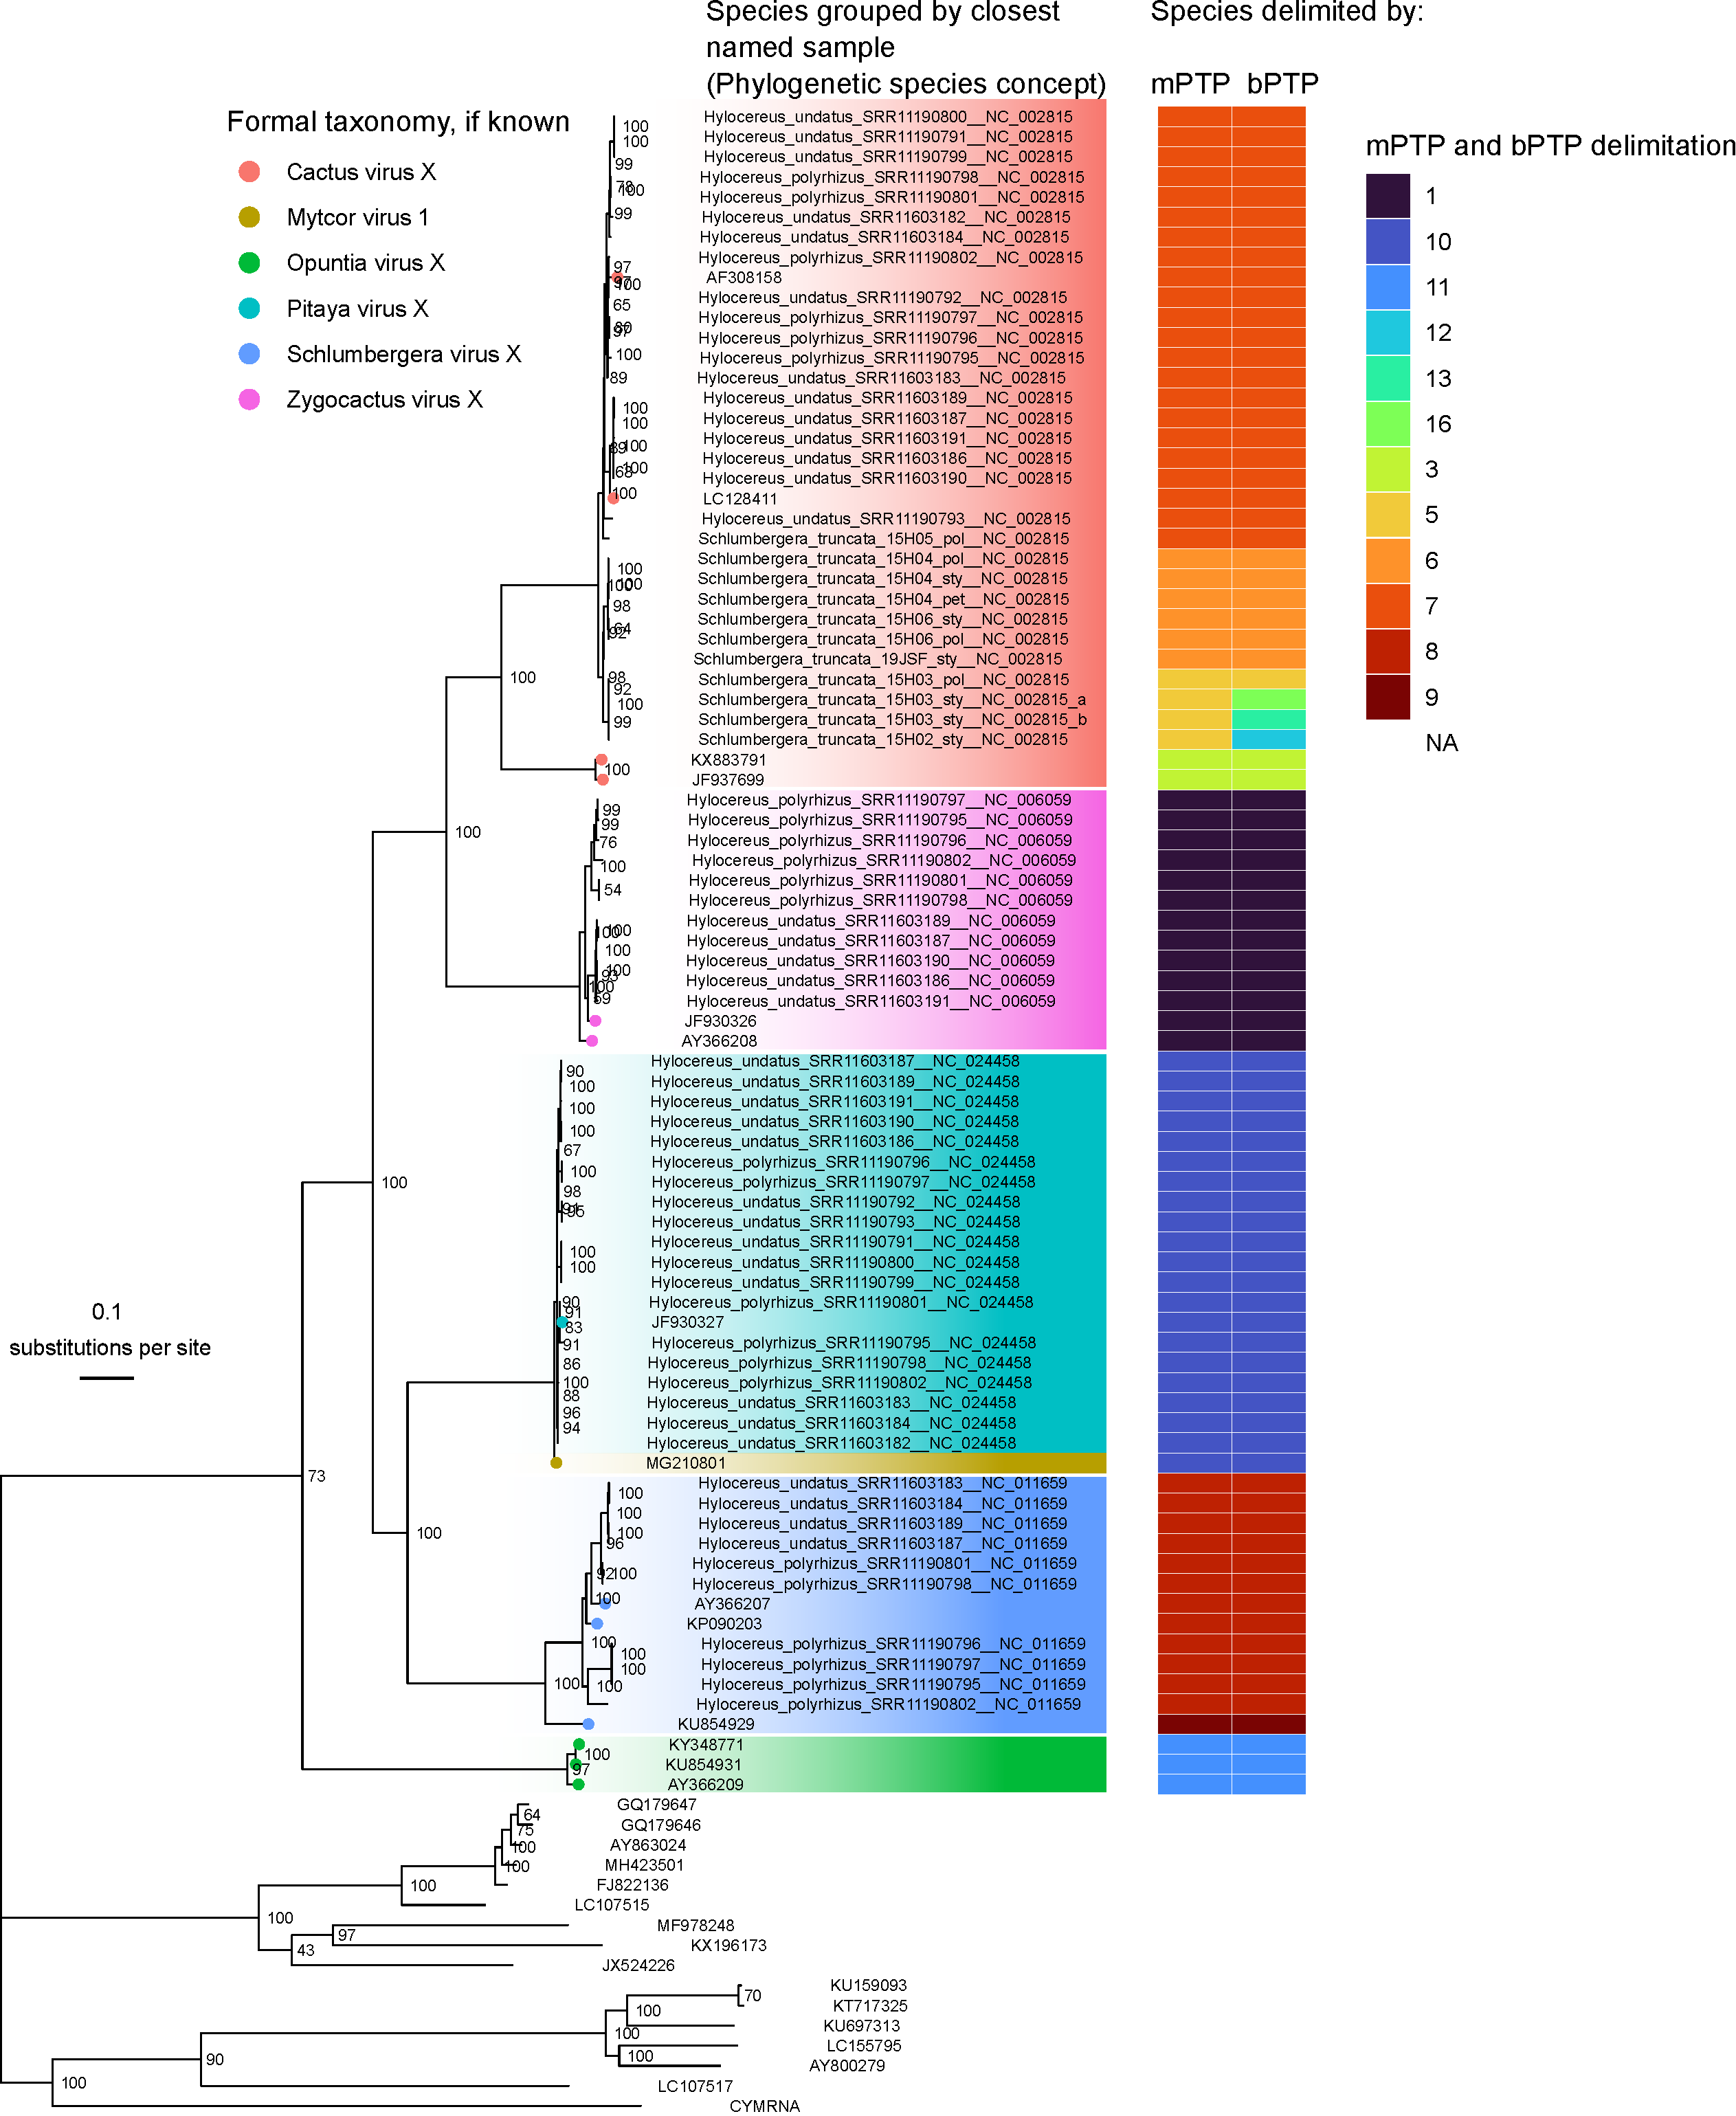
\includegraphics[width=1\linewidth]{figures/delim-edited.pdf}
 \begin{NoHyper}
 \caption{
Maximum likelihood tree for full genome sequences from selected potexviruses. UFboot scores are represented on nodes. Tips are characteristically arranged in large groups with short branches, subtended by a longer branch. This subset of cactus-infecting potexviruses displays narrow sampling across related cohort plants which may represent local viral transmission from plant to plant. The outgroup clade consists of closely related but non-cactus infecting potexviruses.
}
 \label{fig:fig1}
 \end{NoHyper}
 \end{figure}

%%%%%%%%FIGURE 2
\newpage{}
 \begin{figure}[ht]
 \centering
 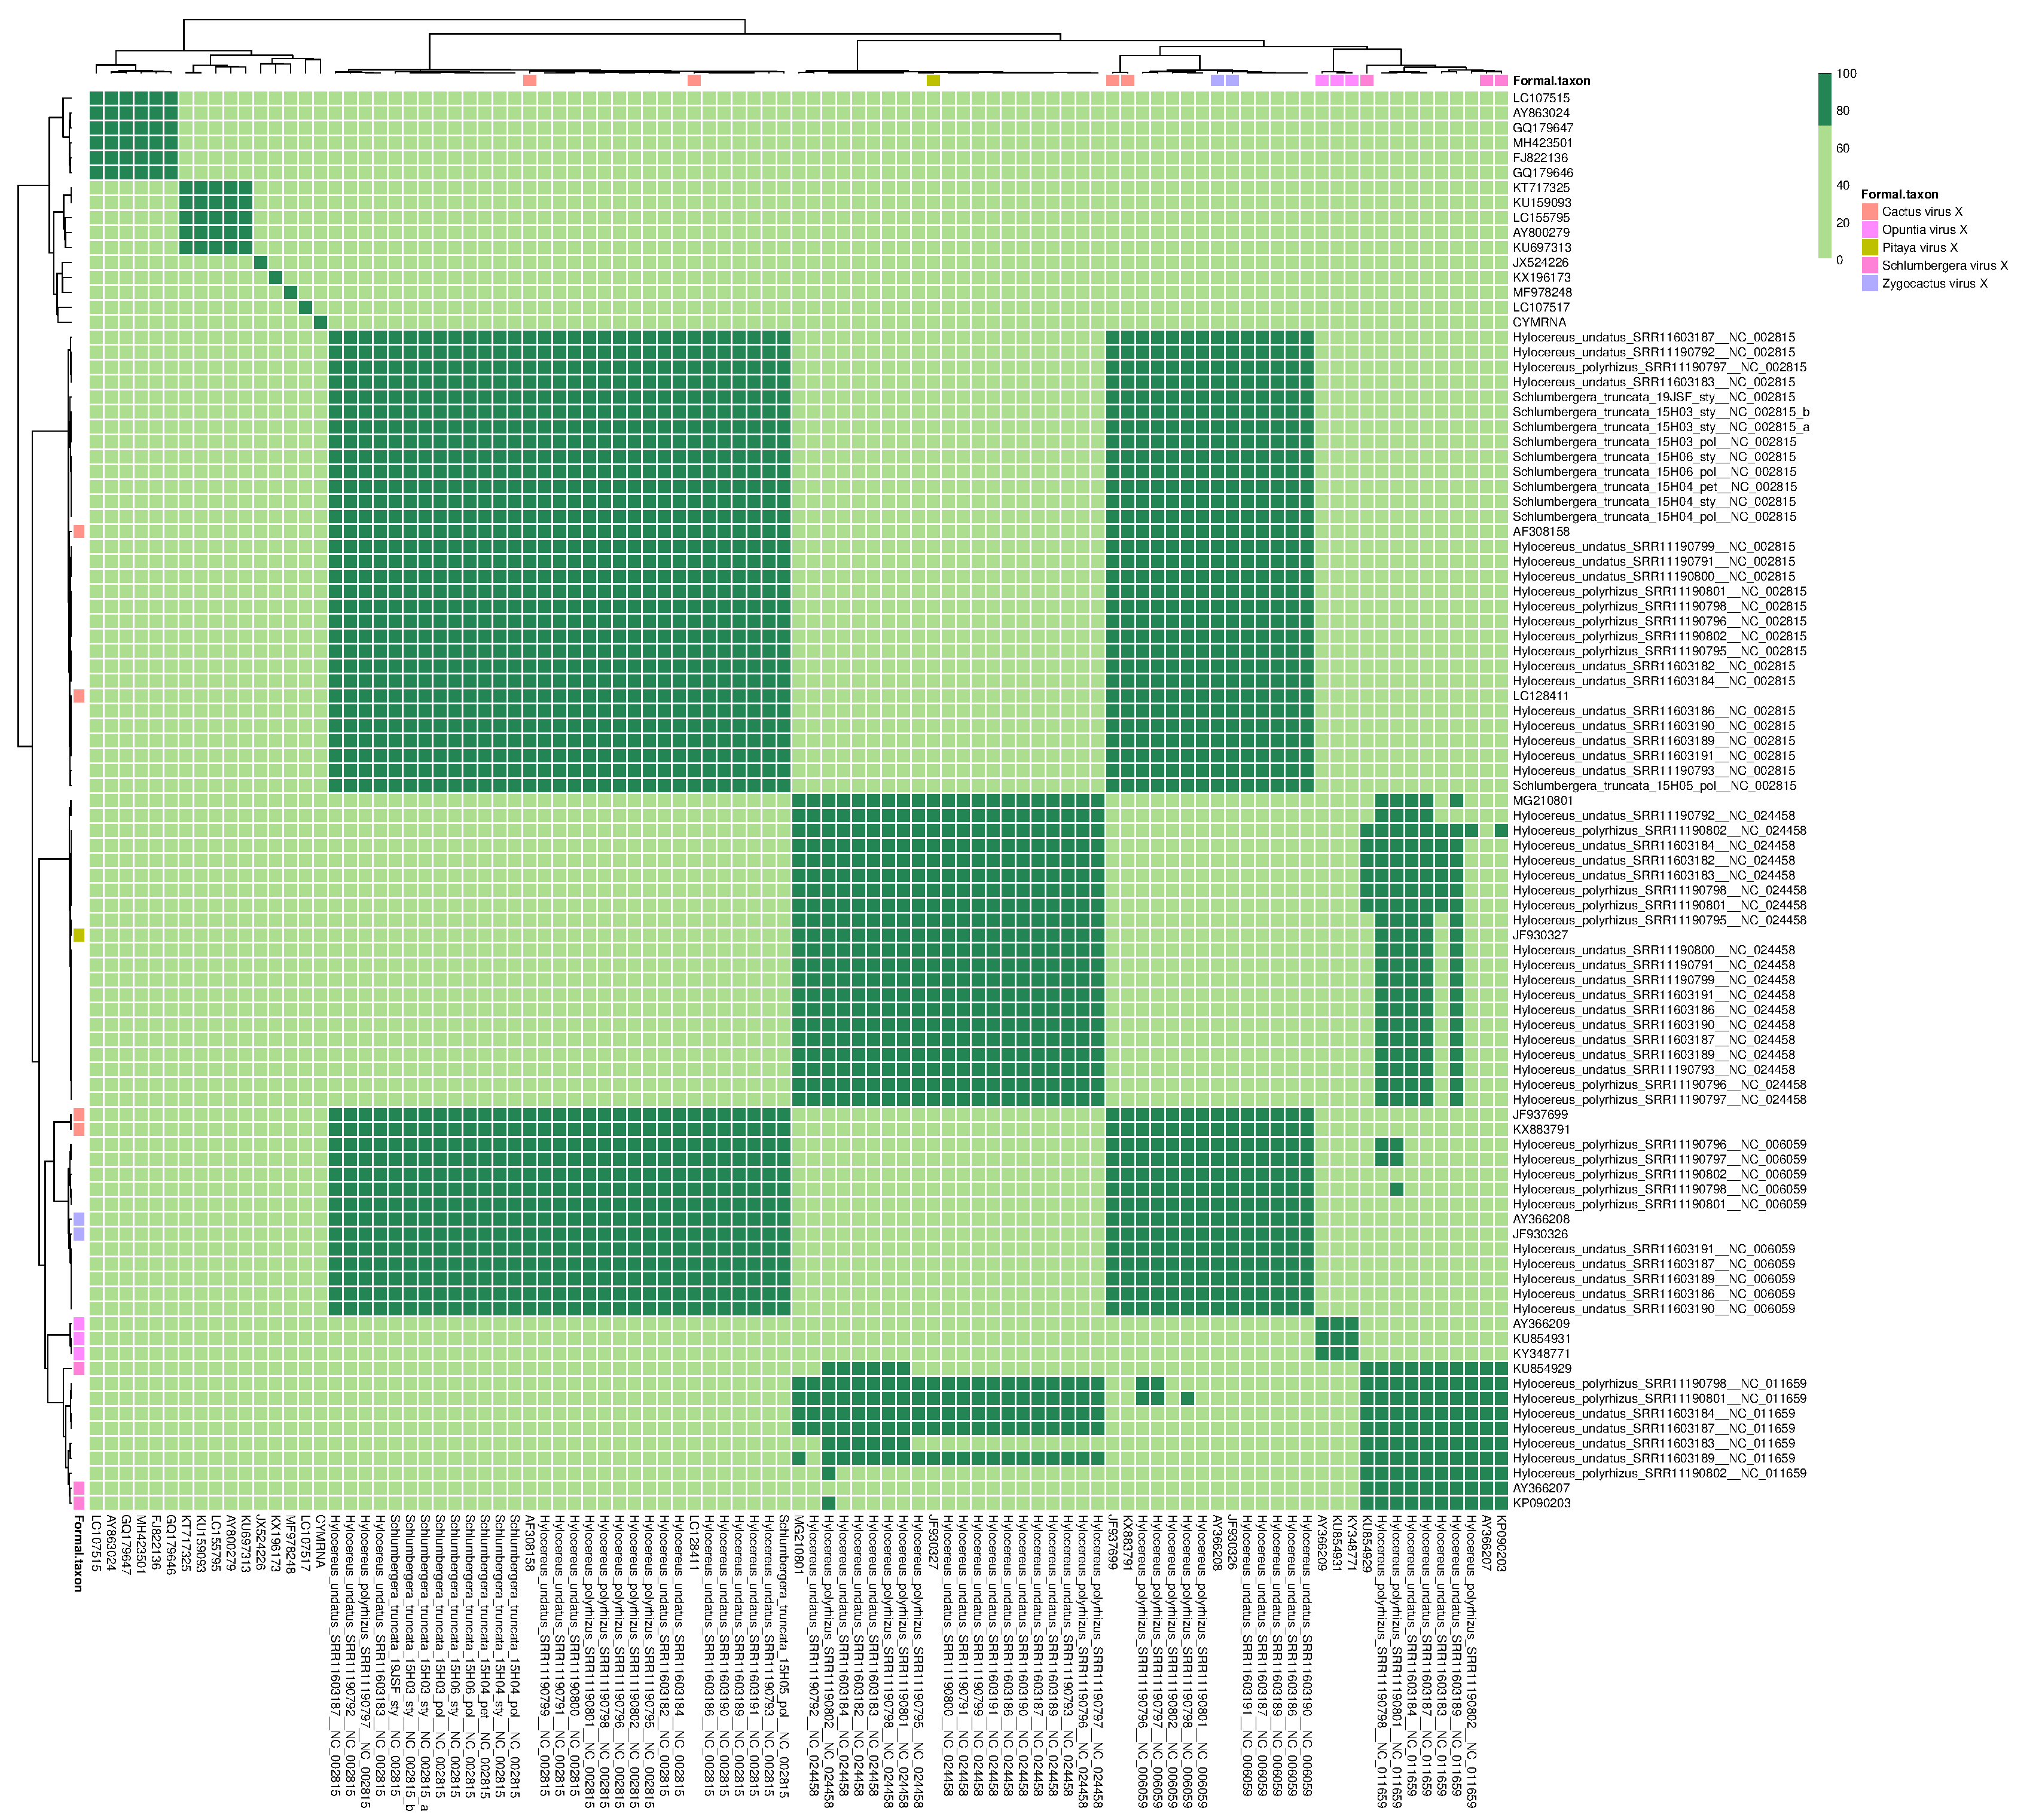
\includegraphics[width=1\linewidth]{figures/heatmap.rdrp.pdf}
 \begin{NoHyper}
 \caption{
Heatmap displaying sequence similarity for aligned ORF1 gene RdRp (RNA-dependent RNA polymerase), which is the largest gene in the potexvirus genome. The genes (n=95) were extracted from each assembled sequence and aligned with MAFFT v7.490 \citep{katoh_mafft_2002}. Sequence similarity percentage was calculated across the 5268 nt aligned sequences in \textit{R} using the \textit{dist.dna} function from ape v. 5.7-1. Darker squares represent areas of higher percentage similarity, and values below the ICTV-suggested 72 percent nt identity are represented in a lighter yellow green.
}
 \label{fig:fig2}
 \end{NoHyper}
 \end{figure}
 
 %%%%%%%%FIGURE 3
\newpage{}
 \begin{figure}[ht]
 \centering
 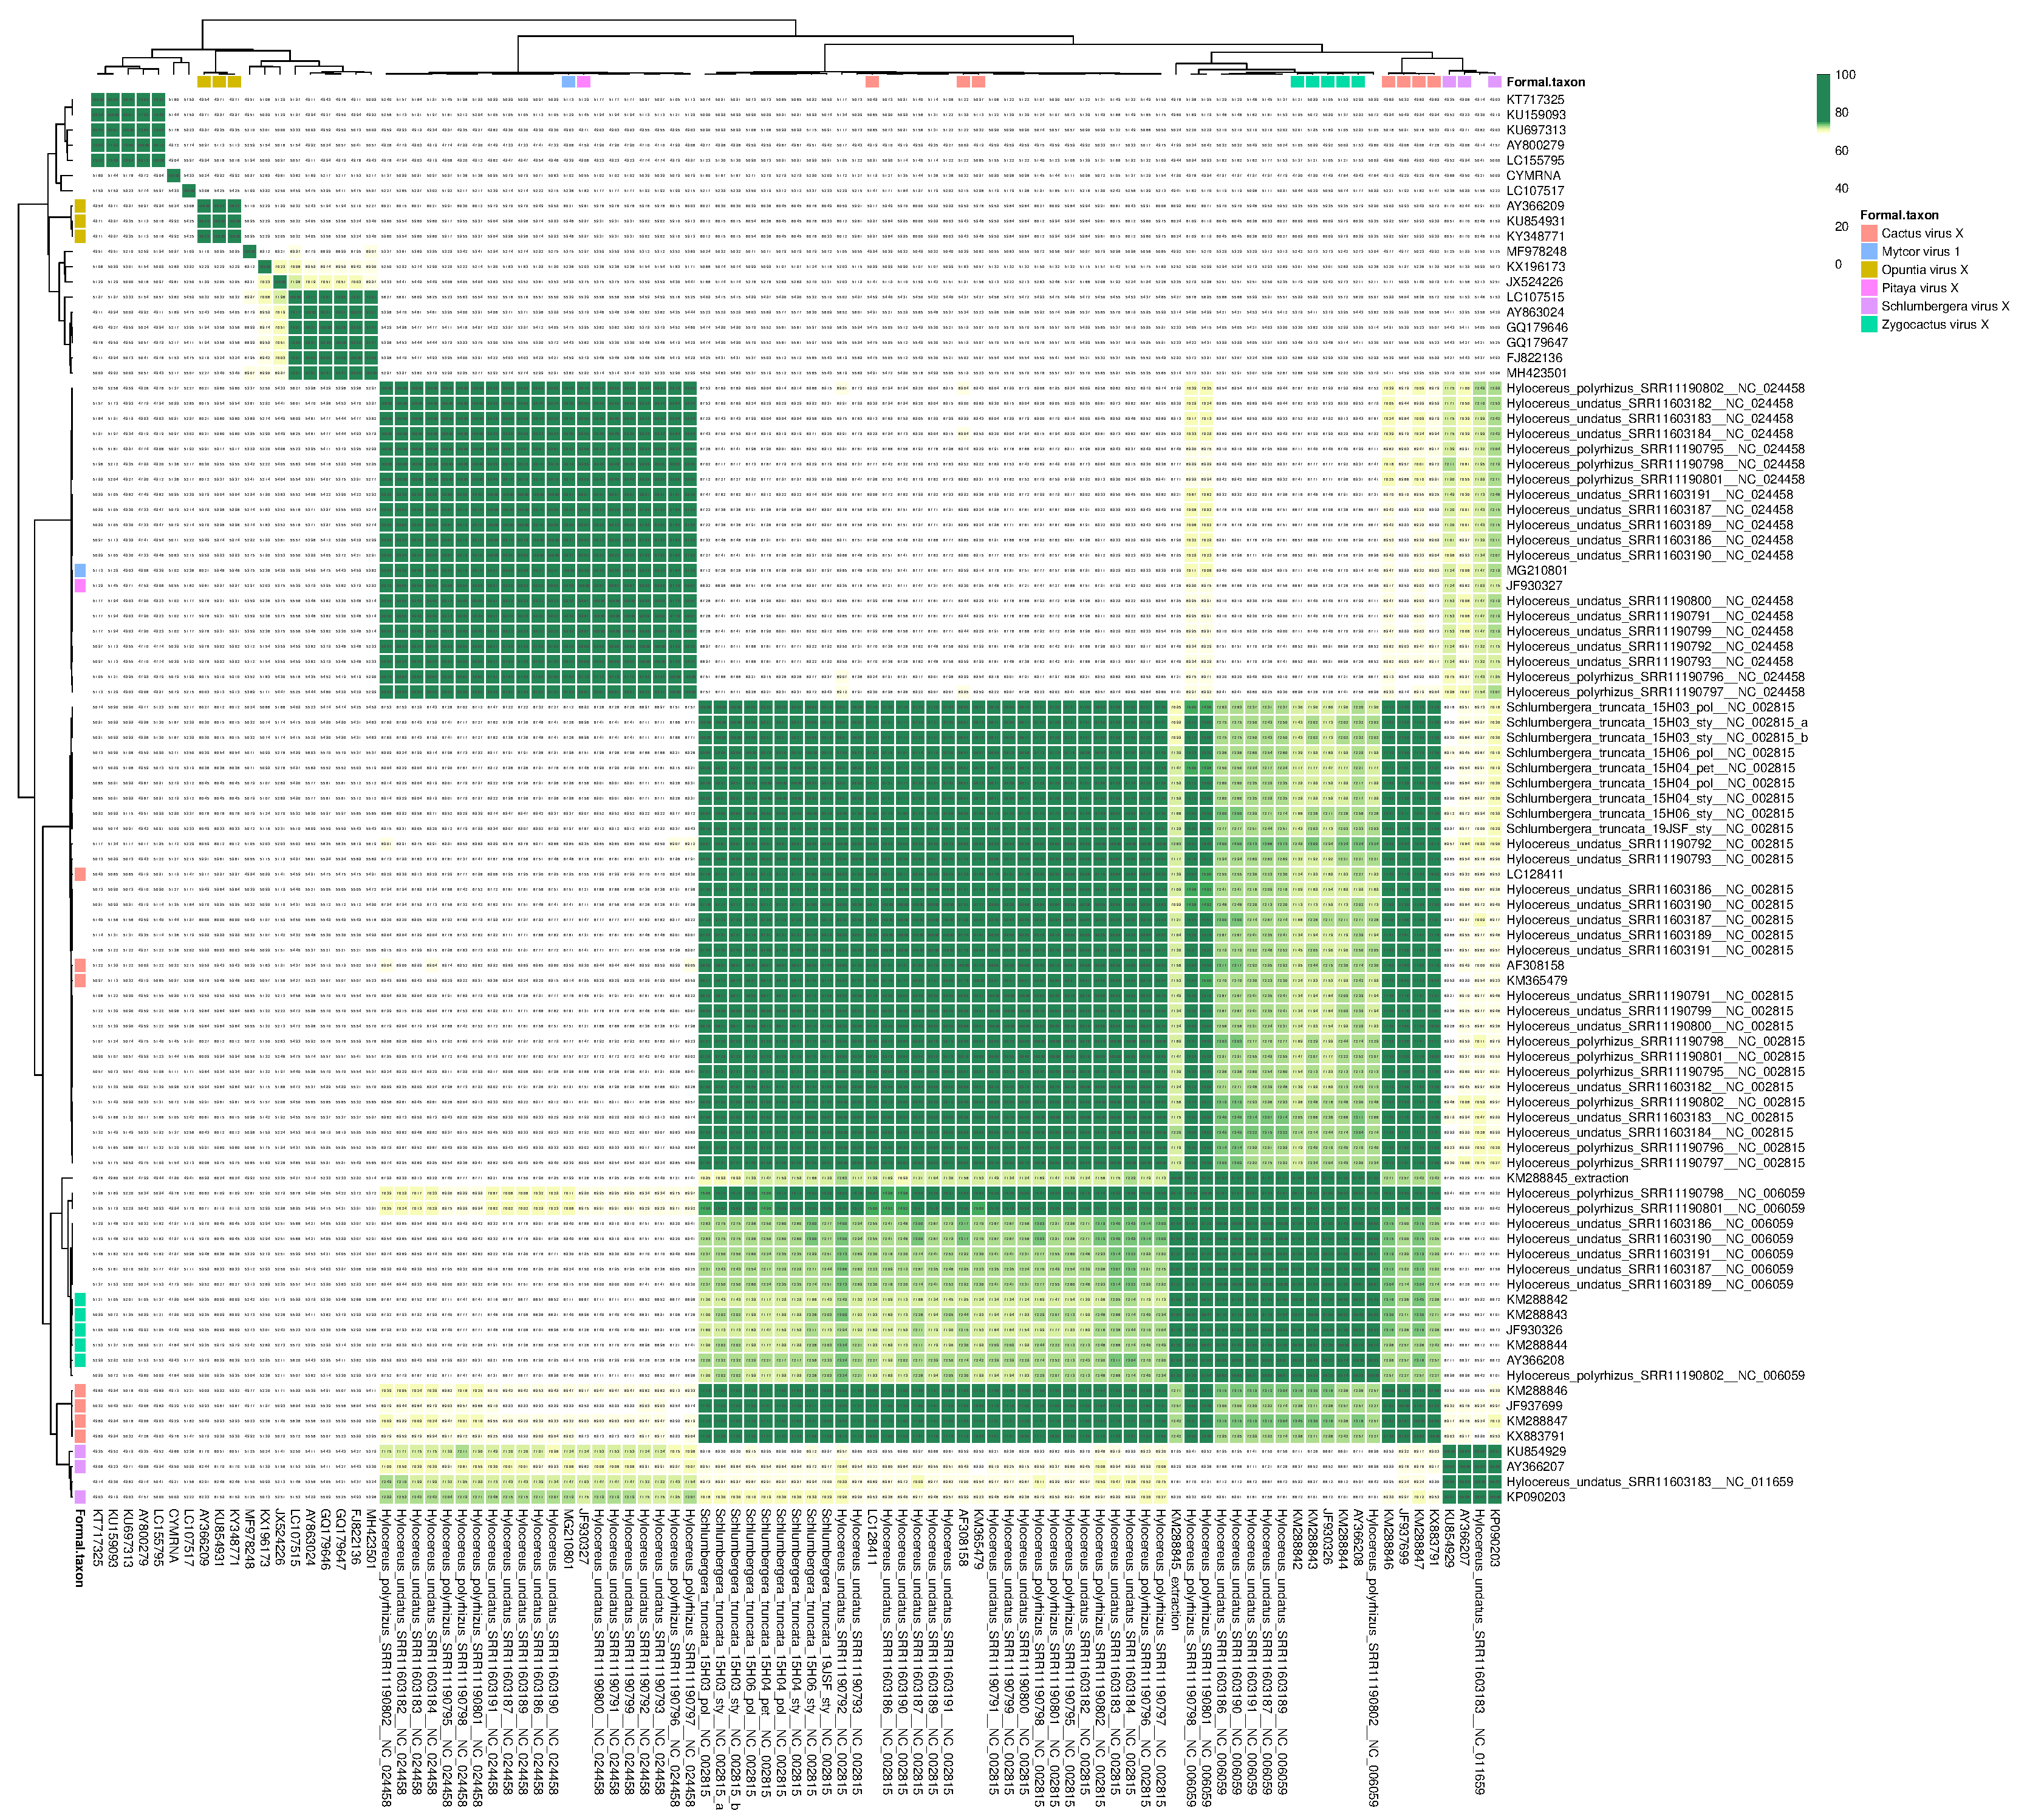
\includegraphics[width=1\linewidth]{figures/heatmap.cp.pdf}
 \begin{NoHyper}
 \caption{
Heatmap displaying sequence similarity for Coat Protein (CP) sequences, using the same coloration as {Figure~2}. CP in potexviruses is typically located in ORF5 and this alignment represents 93 sequences each 714 nt in length.
}
 \label{fig:fig3}
 \end{NoHyper}
 \end{figure}



%%%%%%%%FIGURE 4
\newpage{}
 \begin{figure}[ht]
 \centering
 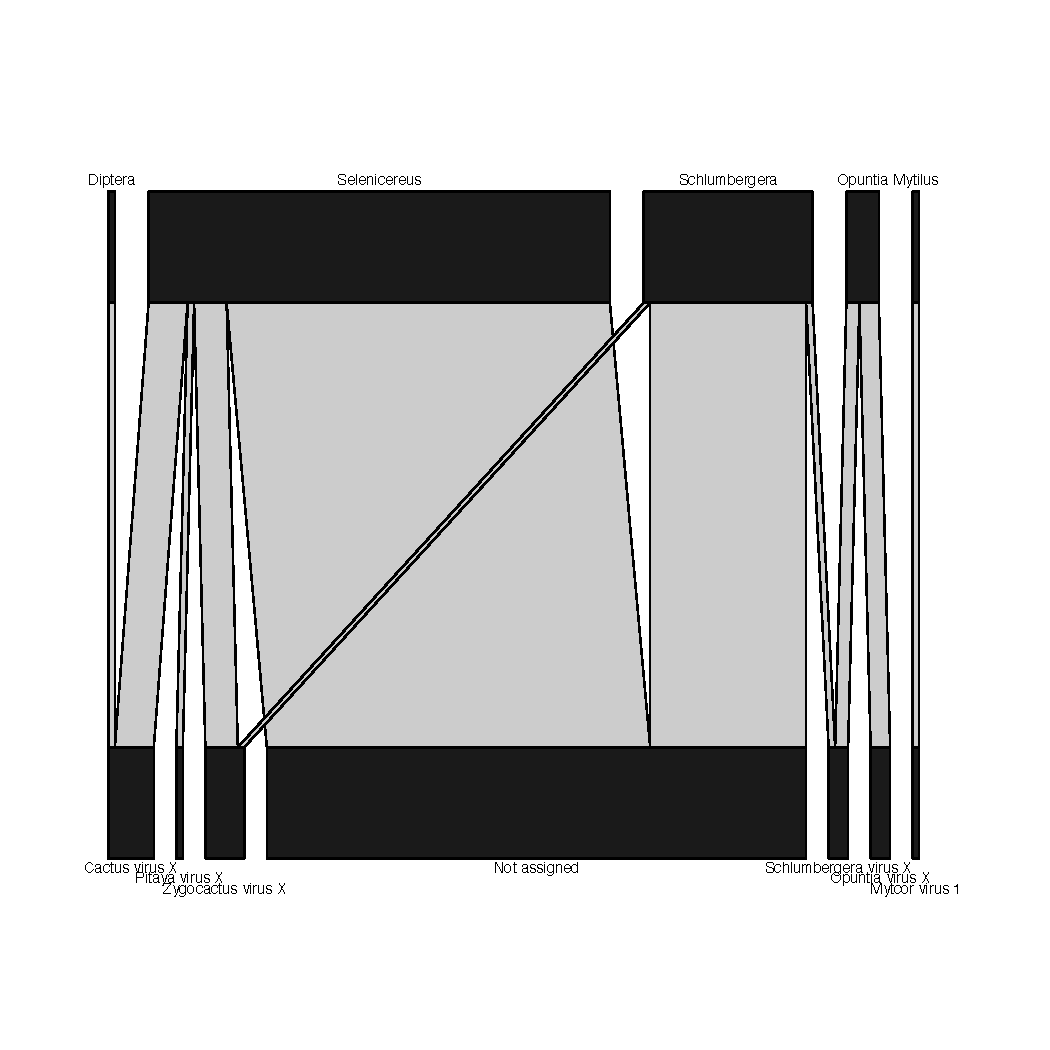
\includegraphics[width=1\linewidth]{figures/hostxformalname.pdf}
 \begin{NoHyper}
 \caption{
Comparing host information to formal viral species name for all samples (n=120) included in our dataset reveals the inconsistencies of viral naming schemes. Delimiting a viral species from its host plant is often an informative first step in viral discovery but may eventually lead to confusion.
}
 \label{fig:fig4}
 \end{NoHyper}
 \end{figure}



% \begin{figure}[ht]
% \centering
% \includegraphics[width=0.5\linewidth]{FILE_PATH}
% \begin{NoHyper}
% \caption{{\fontsize{10pt}{11pt}\selectfont}
% \label{fig:FIG_LABEL}
% \end{NoHyper}
% \end{figure}

% END =========================================================================

\end{document}


%--------------------------------------------------
\section*{To-do and relevant fixes to be completed before submission}
%--------------------------------------------------
\begin{enumerate}
\item Figure captions need to be expanded and proofread.
\item Some methods and results are patchy and need to be written, and they are \hl{highlighted} as a reminder. 
\item The capitalization and italicization of \textit{Potexvirus} is not as consistent as it could be -- I apologize for this nuisance. When referring to the \textit{Potexvirus} genus or using \textit{Potexvirus} as an adjective, it should be capitalized and italicized. As a noun, such as "potexviruses", it is okay uncapitalized and unitalicized.
\end{enumerate}